\section{Efficiency}\label{sec:efficiency}
Another important metric to determine the feasibility of the machine learning model is the efficiency. The main question is if or from what table size the model is faster than a naive method. This becomes even more interesting as each positive guess of the model has to be verified using the naive algorithm because the model is trained for the highest recall and precision, not accuracy. % TODO: ref to model

% TODO: Describe which model where used -> 3 hours, 10.000 tables, recall_precision

\subsection{Experiment Data}\label{subsec:efficiency-experiment_data}
The experiment was conducted on a set of generated tables to control for the size of the table as well as the number of unique and non-unique columns, as can be seen in Table~\ref{table:efficiency-generated_table}.

For the experiments, tables with different sizes were generated. They each had \num{10} columns and between \num{100} and \num{100000000} columns. To ensure the correct prediction by the model, the columns where generated in a specific way. The unique columns are evenly incrementing for the first \num{50} rows, while the first two rows of the non-unique columns contain the same value. The rest of each column contains distinct incrementing values which are mixed up to increase the time of the naive algorithm which works by sorting each column. % TODO: ref to naive algorithm

\begin{table}[!ht]
  {
    \newcommand{\tablevdots}{\multicolumn{1}{c}{\vdots{}}}
    \setlength{\tabcolsep}{5pt}
    \caption[A table generated for the efficiency experiment]{A table generated for the efficiency experiment. The columns 0 and 1 do not contain any duplicates, the columns 2, 3 and 4 do. To guarantee that the model guesses the unique and non-unique columns correctly, the unique columns are evenly incrementing for the first 50 rows, while the duplicate value of the non-unique columns is in the first two rows.}
    \begin{tabularx}{\linewidth}{X<{\centering}SSSSS}
      \toprule
      {Index}       & {Column \num{0}} & {Column \num{1}} & {Column \num{2}} & {Column \num{3}} & {Column \num{4}} \\ \midrule
      \num{0}       & 0                & 0                & 100              & 100              & 100              \\
      \num{1}       & 1                & 1                & 100              & 100              & 100              \\
      \num{2}       & 2                & 2                & 93               & 93               & 93               \\
      \num{3}       & 3                & 3                & 45               & 45               & 45               \\
      % 4        & 4                & 4                & 16               & 16               & 16               \\
      % 5        & 5                & 5                & 87               & 87               & 87               \\
      % 6        & 6                & 6                & 32               & 32               & 32               \\
      \tablevdots{} & \tablevdots{}    & \tablevdots{}    & \tablevdots{}    & \tablevdots{}    & \tablevdots{}    \\
      % 46       & 46               & 46               & 2                & 2                & 2                \\
      % 47       & 47               & 47               & 73               & 73               & 73               \\
      \num{48}      & 48               & 48               & 89               & 89               & 89               \\
      \num{49}      & 49               & 49               & 39               & 39               & 39               \\
      \num{50}      & 91               & 91               & 60               & 60               & 60               \\
      \num{51}      & 77               & 77               & 49               & 49               & 49               \\
      % 52       & 54               & 54               & 23               & 23               & 23               \\
      % 53       & 70               & 70               & 30               & 30               & 30               \\
      \bottomrule{}
    \end{tabularx}\label{table:efficiency-generated_table}

  }
\end{table}



\subsection{Base experiment}\label{subsec:efficiency-base_experiment}
For the first experiment, a model which uses 10 rows as its input was used. The experiment data consisted of \num{9} tables with \num{10} columns each and between \num{100} and \num{100000000} rows. Three of the columns where unique, seven contained duplicates.

Figure~\ref{fig:efficiency-base_experiment-plot} and Table~\ref{table:efficiency_csv-70percent} show that for tables with up to \num{100000} rows, the naive algorithm takes only a fraction of a second and is therefore faster than the proposed machine learning model. However, since the model takes a roughly constant time of half a second, it becomes faster as the table size surpasses one million rows.

Particularly noteworthy is the fact that the validation time for the model takes very close to \SI{30}{\percent} of the time of the naive algorithm. That is because only columns which are unique according to the model are validated, so in this case three.

In conclusion, it is clear that for large tables the most time is used loading the dataset and checking the columns for duplicates with the naive algorithm. While a possible improvement of the naive algorithm is not part of this thesis, in Section~\ref{subsec:efficiency-shorter_loading_times} two different ways to shorten the loading times will be explored. % TODO: write better

\begin{figure}[ht]
  \caption[Compare the efficiency the proposed method and the naive algorithm]{This plot shows the total time for the naive algorithm and the proposed method to compute the unique columns as can be seen in Table~\ref{table:efficiency_csv-70percent}. The tables were saved in a CSV format.} % TODO: better caption
  \label{fig:efficiency-base_experiment-plot} % chktex 24
  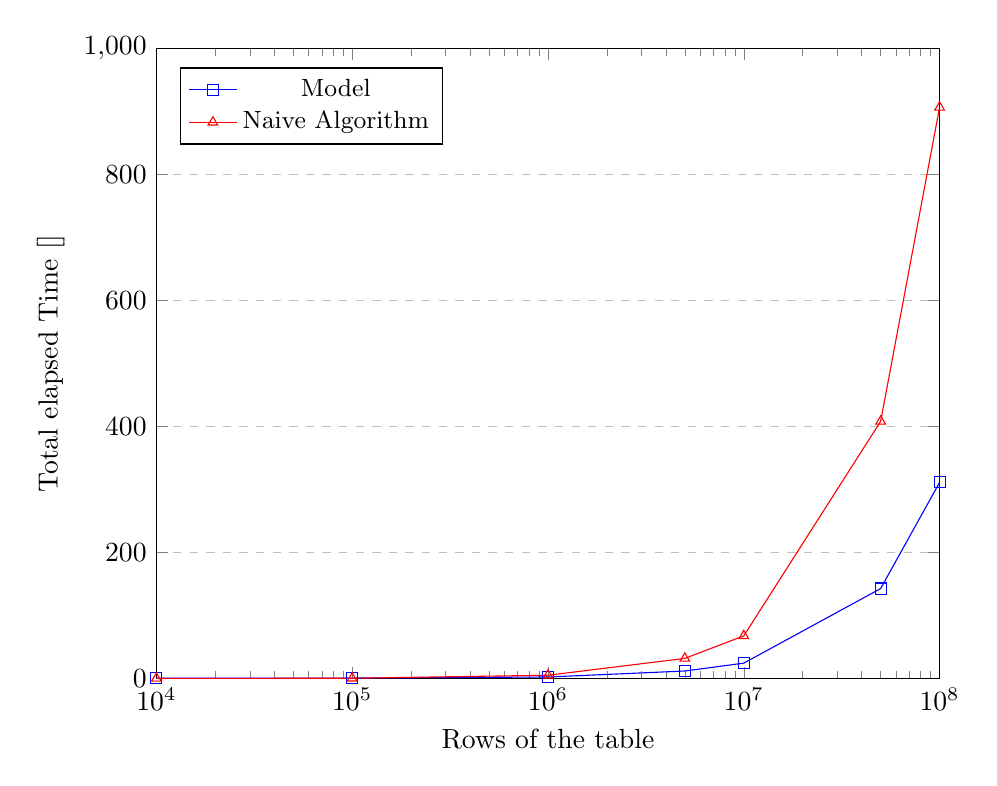
\begin{tikzpicture}
    \begin{axis}[
        % title={},
        xlabel={Rows of the table},
        ylabel={Total elapsed Time [\si{\second}]},
        xmin=10000, xmax=100000000, xmode=log,
        ymin=0, ymax=1000,
        % xtick={0,1000,100000,10000000,100000000},
        % ytick={0,20,40,60,80,100,120},
        legend pos=north west,
        ymajorgrids=true,
        grid style=dashed,
        scale only axis,
        width={\linewidth-62pt},
        height=8cm
      ]

      \addplot[
        color=blue,
        mark=square,
      ]
      coordinates {
          (100.0,1.0835406184196472) (1000.0,0.4514627978205681) (10000.0,0.4591604061424732) (100000.0,0.5741918832063675) (1000000.0,2.2600879333913326) (5000000.0,11.771335251629353) (10000000.0,24.25790297240019) (50000000.0,142.64984269440174) (100000000.0,311.1732710637152)
        };
      \addplot[
        color=red,
        mark=triangle,
      ]
      coordinates{
          (100.0,0.0039823874831199) (1000.0,0.0037141181528568) (10000.0,0.0264939442276954) (100000.0,0.3022922314703464) (1000000.0,5.0495885498821735) (5000000.0,31.796920645982027) (10000000.0,67.54112743958831) (50000000.0,408.1332451477647) (100000000.0,906.6464131213723)
        };
      \legend{\small Model, \small Naive Algorithm}

    \end{axis}
  \end{tikzpicture}
\end{figure}



\subsection{Shorten loading times}\label{subsec:efficiency-shorter_loading_times}
While CSV files are very easy to use, they are not meant to efficiently store large quantities of data. A file format which is substantially more suitable to handle large datasets is the parquet format\cite{parquet-book}.

It achieves this through the use of various features such as column wise compression, which tends to be more efficient since the values in the same column are usually very similar. This has the additional benefit of enabling the algorithm to only read the required columns which may decrease \io{} as only positive guesses need to be loaded for the validation.

Another advantageous property of this format is the concept of row groups, which ensure that a batch of rows is being saved together and can therefore be read together too. This makes it possible to read just the first row group and use these rows as an input for the model.

The Table~\ref{table:efficiency_parquet-70percent} shows the result of the base experiment from Section~\ref{subsec:efficiency-base_experiment} repeated with tables generated as parquet files. While the computing time for the model and the naive algorithm remain roughly equal compared to Table~\ref{table:efficiency_csv-70percent}, the loading time is decreased significantly for large tables. %? loading times make up a larger part of total time for model

Table~\ref{table:efficiency_parquet-70percent_small-tables} presents the result for the experiment using the advantages of the file format by loading only the necessary rows and columns. That is why in this case, there are two loading times for the model. The first time only the first row group is being loaded while the second time only the columns which are unique according to the model are loaded for validation. However, this does not make any difference except for the largest table and even then the total time is hardly changing.

In summary, although the reduced \io{} does make a notable difference, it is not very large compared to the efficiency gain through the use of the model, as can be seen in Figure~\ref{fig:efficiency-shorter_loading_time-plot}. This could change, however, if the file reading speed would be slower, for example because they have to be read over the internet. In this case, reading only the necessary rows and columns could make a larger difference too.

\begin{figure}[ht]
  \caption[]{} %! TODO: better caption
  \label{fig:efficiency-shorter_loading_time-plot} % chktex 24
  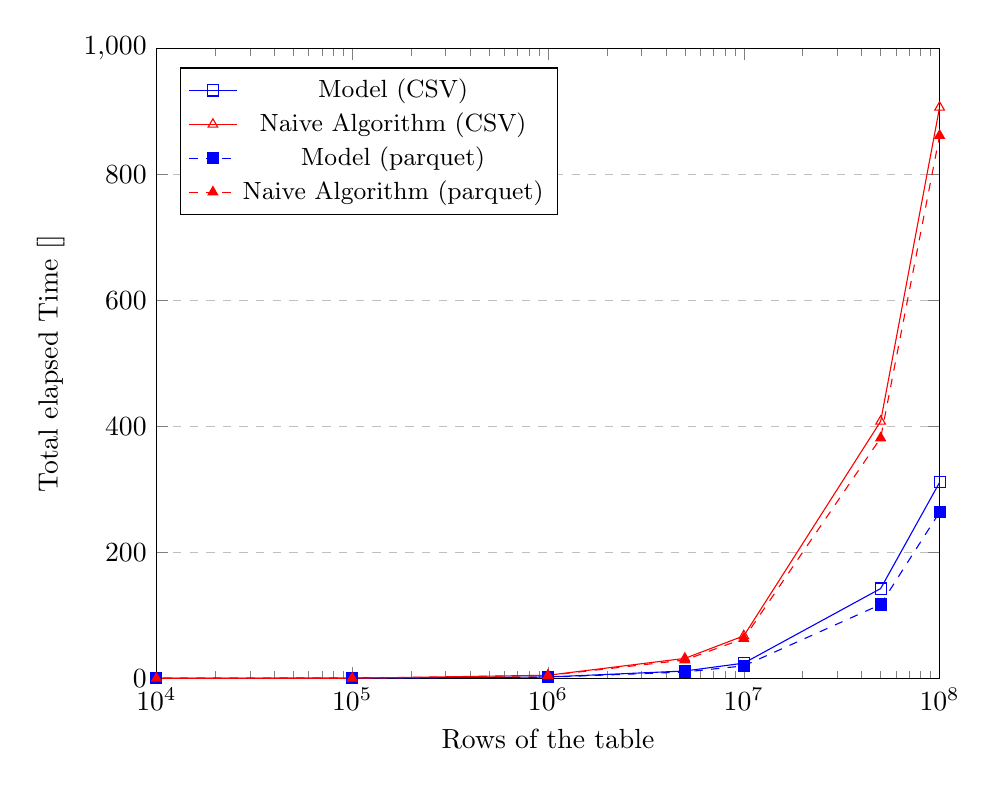
\begin{tikzpicture}
    \begin{axis}[
        % title={},
        xlabel={Rows of the table},
        ylabel={Total elapsed Time [\si{\second}]},
        xmin=10000, xmax=100000000, xmode=log,
        ymin=0, ymax=1000,
        % xtick={0,1000,100000,10000000,100000000},
        % ytick={0,20,40,60,80,100,120},
        legend pos=north west,
        ymajorgrids=true,
        grid style=dashed,
        scale only axis,
        width={\linewidth-62pt},
        height=8cm
      ]

      % csv
      \addplot[
        color=blue,
        mark=square,
      ]
      coordinates {
          (100.0,1.0835406184196472) (1000.0,0.4514627978205681) (10000.0,0.4591604061424732) (100000.0,0.5741918832063675) (1000000.0,2.2600879333913326) (5000000.0,11.771335251629353) (10000000.0,24.25790297240019) (50000000.0,142.64984269440174) (100000000.0,311.1732710637152)
        };

      \addplot[
        color=red,
        mark=triangle,
      ]
      coordinates{
          (100.0,0.0039823874831199) (1000.0,0.0037141181528568) (10000.0,0.0264939442276954) (100000.0,0.3022922314703464) (1000000.0,5.0495885498821735) (5000000.0,31.796920645982027) (10000000.0,67.54112743958831) (50000000.0,408.1332451477647) (100000000.0,906.6464131213723)
        };

      % parquet
      \addplot[
        color=blue,
        mark=square*,
        dashed,
        mark options={solid}
      ]
      coordinates {
          (100.0,0.4577647559344768) (1000.0,0.4482727721333504) (10000.0,0.4571339413523674) (100000.0,0.5343325138092041) (1000000.0,1.90179156512022) (5000000.0,10.232811015099289) (10000000.0,19.938058882951736) (50000000.0,117.29449190944432) (100000000.0,263.89783180877566)
        };

      \addplot[
        color=red,
        mark=triangle*,
        dashed,
        mark options={solid}
      ]
      coordinates{
          (100.0,0.0062335357069969) (1000.0,0.0053194314241409) (10000.0,0.0245211236178874) (100000.0,0.2559473849833011) (1000000.0,4.6651470102369785) (5000000.0,29.216464921832085) (10000000.0,63.27469082176685) (50000000.0,381.673400811851) (100000000.0,861.8326124921441)
        };

      %       % parquet small_table
      %       \addplot[
      %         color=blue,
      %         mark=square,
      %       ]
      %       coordinates {
      % (100.0,0.4629099182784557) (1000.0,0.4608258455991745) (10000.0,0.4631855227053165) (100000.0,1.5644594952464104) (1000000.0,1.8686350099742413) (5000000.0,9.371084868907928) (10000000.0,19.90878576785326) (50000000.0,117.83388417959212) (100000000.0,261.4674338325858) 
      % };

      %       \addplot[
      %         color=red,
      %         mark=triangle,
      %       ]
      %       coordinates{
      % (100.0,0.0039786621928215) (1000.0,0.0044715628027915) (10000.0,0.024229060858488) (100000.0,0.2556539326906204) (1000000.0,4.715674605220556) (5000000.0,29.195809934288263) (10000000.0,63.66628506034613) (50000000.0,381.9564390294254) (100000000.0,861.1740412451327) 
      % };

      \legend{\small Model (CSV), \small Naive Algorithm (CSV), \small Model (parquet), \small Naive Algorithm (parquet)}

    \end{axis}
  \end{tikzpicture}
\end{figure}



\subsection{Comparing models with different input sizes}\label{subsec:efficiency-comparing_models} % TODO: Writing
Short description of what \enquote{different input sizes} means (long explanation in earlier section).

Compare times for \SI{70}{\percent}.

Conclusion: No large difference, the difference may correlate with the larger file size of the model itself.


\subsection{Changing the ratio of unique columns}\label{subsec:efficiency-changing_uniques} % TODO: Writing
Description of the experiment setup: Parquet with small table and 60, 70, 80, 90\%.

Description of what is happening.

What percentage of unique columns in the gittables dataset?

Conclusion: The increased efficiency depends mainly on the low fraction of unique columns (next to number of rows). Probably is the real world percentage low enough.


\subsection{Summarized results}\label{subsec:efficiency-summarized_results} % TODO: Writing
The proposed model is more efficient for large enough tables. The percentages are good enough in the real world. Only loading necessary rows/columns has not been a large advantage in this case, but it could be with slow \io{}.
